\section{Introduction}
In this section the workflow and results of the User Testing phase are presented and discussed.

This phase required asking new users to surf on the UNICEF and complete a series of tasks while being observed, with little to no intervention or help, by the inspectors. The main objective was to confirm the critical flaws and issues detected during the Inspection phase and discover new ones thanks to the unpredictability of behavior of the tester.

\section{Design of the study}
User Testing requires a setup phase where choices are made on who the testers should be, what should they test and why should they test it. Following is a brief discussion on such phase.

\subsection{User profiles}
The following is the user profile we agreed to target for the purpose of this testing phase: people in their 20s which are involved with or interested in politics and social matters.

During the inspection, it became clearer who are the users the website is targeting when delivering so much information: these are people deeply interested in social matters and crisis and the consequences that these might have on children also. UNICEF wants to share as much details as possible to its audience to convince them to either \textbf{donate} or \textbf{take part} as volunteers or workers willing to help with the agency's operations around the world.

We specifically decided not to include any constraint regarding technical knowledge into the user profile, to make this activity open to a broader group of people. Later on we will discuss how such decision brought us to interesting results, data and behavior by the testers.

\subsection{Tasks}
In the previous chapter, we highlighted a set of heuristics and questions that failed to score an average higher than \textbf{2,5} points out of 5. We present them here for simplicity:
\begin{itemize}
	\item \textbf{N1.2} Does the website provide breadcrumbs to define the user position?
	\item \textbf{N3.2} Does the website allow the user to correctly navigate back to a previous section or page?
	\item \textbf{N4.1} Is the website consistent with wording, visual and routing elements?
	\item \textbf{N7.1} Does the website offer shortcuts to common functions?
	\item \textbf{N7.2} Does the website allow customization and personalization of interaction, catering to both expert and novice users?
	\item \textbf{N8.1} Is the website exempt from unnecessary information or links?
	\item \textbf{N10.1} Is the documentation of the website, when provided, searchable and navigable?
	\item \textbf{MN1} Do pages of the same type have the same navigation links and interaction capability?
	\item \textbf{MN2} It is easy to navigate from/among groups of “items”, and within the items?
\end{itemize}

Starting from such result, we designed the following tasks to try to tackle such flaws in the usability of the website, to check whether the testers would obtain the same results. We decided to provide the tester with a \textbf{context or scenario}, which would help the tester contextualize the task, and the \textbf{task} the testers would be asked to complete.

For each task we also decided on a time limit, over which the task would be considered not completed. Also an error count has been tracked during the testing. We realized an error limit was not ideal for the evaluation of this website, so while we tracked it, it was scrapped from the discussion of the results.

Table \ref{tab:task_details} details the tasks and the associated scenarios and time limits:

\begin{longtable}{|>{\RaggedRight}m{0.5\linewidth}|>{\RaggedRight}m{0.3\linewidth}|>{\RaggedRight}m{0.1\linewidth}|}
    \caption{Tasks details} \label{tab:task_details}\\
    \hline
    \multicolumn{3}{|c|}{\textbf{MiLE (Navigation) Heuristics' Final Scores}} \\
    \hline
    \textbf{Scenario} & \textbf{Task} & \textbf{Time Limit} \\
    \hline
    \endfirsthead
    \multicolumn{3}{c}
    {\tablename\ \thetable\ -- \textit{Continued from previous page}} \\
    \hline
    \multicolumn{3}{|c|}{\textbf{Tasks details}} \\
    \hline
    \textbf{Inspector} & \textbf{Score} & \textbf{Time Limit}\\
    \hline
    \endhead
    \endfoot
    \hline
    \endlastfoot

\hline
\textbf{1} You are interested in the crisis in DRC (Democratic Republic of Congo) and what to donate a specific amount to the cause. Try to donate to the specific cause of DRC. & Donate to DRC cause & 10m:00s  \\
\hline

\textbf{2} Now you also want to learn more about the conflict in Gaza and want to find out how you could help (by donating). However you also want to make sure you know how your donation is going to be used. Try to donate to the specific cause of DRC. & Donate to Gaza cause and learn what the donation is used for & 05m:00s  \\
\hline

\textbf{3} Imagine you decided to put your effort into volunteering and wanted to apply to do so with Unicef. You want to find information about the application process and the type of job you can volunteer for. & Reach the Samia Aboni page and learn the role & 05m:00s  \\
\hline

\textbf{4a} Suppose you're doing a research about children rights so you navigate the UNICEF website to find at least 3 topics on the subject. & Find at least 3 pages on the Children Rights' topic. & 10m:00s  \\
\hline

\textbf{4b} Once you found the articles, you figure you should also specify human rights in general. & Find an exhaustive list of the human rights on the website. & 05m:00s  \\
\hline

\end{longtable}

\section{Execution of the study}
\subsection{Inspection sheet}
To deliver the test to the testers and gather data, insights and comments, we developed another Google Form, and linked it to a Google Sheet page to make data review easier. This form was divided into varios sections as well:
\begin{itemize}
	\item Data about the tester;
	\item A section for each Task;
	\item System Usability Scale section;
	\item Comments section;
\end{itemize}
We designed the sheet to be used by the inspectors only until the SUS section. At that point, if possible, the user was allowed to reply on their own to the remaining questions through the same form instance.

Each section, as suggested by Figure \ref{fig:testing_form}, would present detailed instruction for the inspector to follow. For instance, we would provide the scenario and task descriptions to explain to the user and add notes visible to the inspector only about the objective of the task and possible error or critical actions that the tester could make.

\begin{figure}[h]
	\centering
	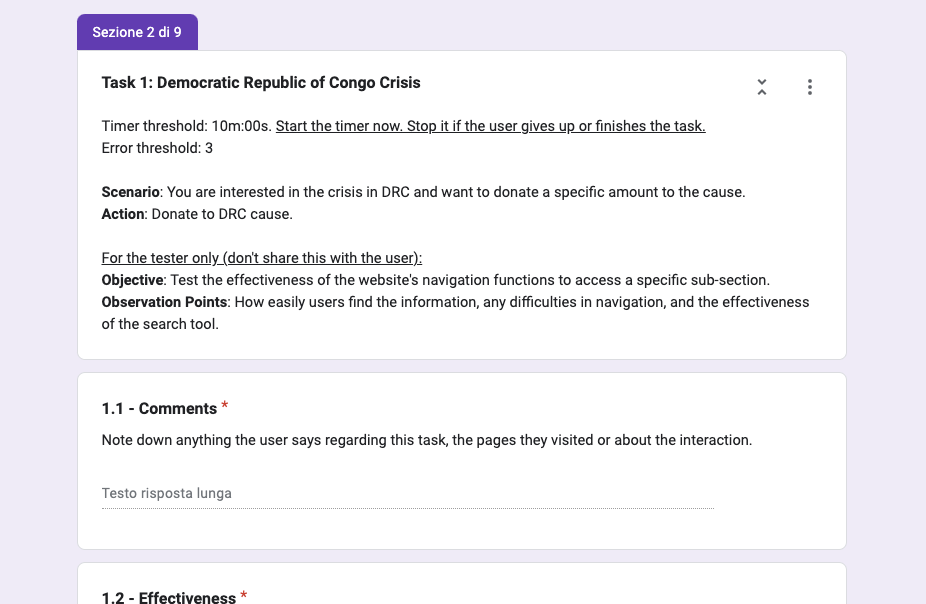
\includegraphics[width=0.8\textwidth]{img/testing_form.png}
	\caption{User Testing form - notice that in this form User refers to the Tester, while the tester is the Inspector.}
	\label{fig:testing_form}
\end{figure}

\subsection{Scale and scores}
Through the form, we collected data regarding the following metrics:
\begin{itemize}
	\item \textbf{Effectiveness} Whether the task was completed and how. We decided the following set of scores to assign based on the outcome of the task:
		\begin{itemize}
			\item \textbf{1} The tester completed the task successfully without need for help or guidance.
			\item \textbf{0.5} The task was completed but assistance was given to do so.
			\item \textbf{0} The task was NOT completed because either the user gave up or the timer expired.
		\end{itemize}
	\item \textbf{Efficiency} The time taken to complete the task.
	\item \textbf{Errors} Number of errors made by the tester.
	\item \textbf{Perceived difficulty} How hard did the tester find the task. In this case we used the usual 1-5 scale, the same we used to evaluate during the Inspection phase.
\end{itemize}

For each task, the tester was asked to think aloud and report anything unusual in their testing phase. A comment field for each task section allowed us to record the flow of operation of the tester, any thoughts they wanted to share and comments in general.

Finally, the System Usability Scale method has been implied to gather further feedback by the testers about the usability of the website. The questions were the following:
\begin{itemize}
	\item \textbf{SUS1} I think I would like to use this application frequently.
	\item \textbf{SUS2} I found the application unnecessarily complex.
	\item \textbf{SUS3} I would imagine that most people would learn to use this application very quickly.
	\item \textbf{SUS4} I thought the application was easy to use.
	\item \textbf{SUS5} I think that I would need the support of a technical person to be able to use this application.
	\item \textbf{SUS6} I found the various functions in this application were well integrated.
	\item \textbf{SUS7} I thought there was too much inconsistency between interactions in the application.
	\item \textbf{SUS8} I found the application very cumbersome to use.
	\item \textbf{SUS9} I felt very confident using the application.
	\item \textbf{SUS10} I needed to learn a lot of things before I could get going with this application.
\end{itemize}

From these answers, the SUS score can be computed for each user, and then the SUS average score can be computed.

\subsection{Testing environment}
We were able to find 19 people that matched our user profile. The activity was executed either online or in-presence. The user could use whatever devices they would see fit, with the only constraint of it being able to display the website in desktop mode. This means that basically only iPads and Laptops were allowed. Each tester would receive an extensive list of instruction regarding the activity and guidance when moving between tasks. Throughout the tasks, the inspector would record any useful information or comment on the inspection sheet.

\section{Results}
\subsection{Final scores}
Figure \ref{fig:background_pie} shows the overall background of the testers' group, while Figures \ref{fig:effec_chart}, \ref{fig:effic_chart}, \ref{fig:perc_eff_chart} show the aggregated scores per-task.

\begin{figure}[h]
	\centering
	\includesvg[width=0.7\textwidth]{img/svg/background_pie.svg}
	\caption{Testers' background}
	\label{fig:background_pie}
\end{figure}

\begin{figure}[h]
	\centering
	\includesvg[width=0.7\textwidth]{img/svg/effectiveness_chart.svg}
	\caption{Successes per-task (Effectiveness)}
	\label{fig:effec_chart}
\end{figure}

\begin{figure}[h]
	\centering
	\includesvg[width=0.7\textwidth]{img/svg/efficiency_chart.svg}
	\caption{Average effectiveness per-task}
	\label{fig:effic_chart}
\end{figure}

\begin{figure}[h]
	\centering
	\includesvg[width=0.7\textwidth]{img/svg/perceived_effort_chart.svg}
	\caption{Average perceived difficulty per-task}
	\label{fig:perc_eff_chart}
\end{figure}

\subsection{SUS score}
Figure \ref{fig:sus_result} shows the result scored by each tester in the SUS section:
\begin{figure}[h]
	\centering
	\includesvg[width=0.9\textwidth]{img/svg/SUS.svg}
	\caption{SUS results per-user and average SUS score}
	\label{fig:sus_result}
\end{figure}
The average SUS score is \textbf{45 points} which means the website has strong usability issues among all testers, which is consistent with the results and the comments by the testers.

\subsection{Comments}
While carrying out the User Testing we have noticed a couple of interesting things about the aspects that most influenced the users' experiences with the website. For each of the tester we collected some general information
about their gender, their age and their field of studies or work. Of these three aspects the one that affected the most the user's results was the background (Figure \ref{fig:background_pie}), whereas gender didn't impact significantly and ages were in a range compliant with the profile of the user persona we picked.
This distinction was particularly noticeable in the way the users would approach the website: while people who had a less technical background and were not too familiar with common practice in web development were more prone to browsing the actual content and reading through it to find what they were searching for, using an approach that could be defined as "explorative". Those with a technical background, however, were overall less patient and felt frustrated when their expectations about elements the website were not met.
As a direct consequence of this specific difference in behavior, the first would most likely complete the tasks perceiving them as easy, while the latter would find convoluted ways to get to the same goal and feel frustrated.

Another consideration to be made about the testing was the learning curve of the users. It's particularly evident by the difference in the time it took them to reach their goals on the first task with respect to the latter.
This means that the more the user familiarized with the website and with the type of task, the faster their navigation became.

\section{Conclusions}
One of the missions of UNICEF is to reach as many people as possible in order to bring them closer to their cause and receive their support. Sadly, given the convoluted nature of the website and its severe inconsistencies, it discourages new users from utilizing it, rather than invite them.
The frustration about the missed expectations of interactions of the users and the overwhelm given by the massive amount of ill-organized content reduces the user's desire to support and to get involved, and results in a great loss of the Agency.
